\documentclass[a4paper]{report} % Formato plantilla

\usepackage{graphicx}
\usepackage[utf8]{inputenc} % Para poder usar caracteres especiales
\usepackage[spanish]{babel} % Para poder usar caracteres especiales

\begin{document} % Inicio del documento Template
  \begin{titlepage}
    \centering
    {\scshape\LARGE Universidad Católica de Pereira\par}
    \vfill
    {\scshape\LARGE Convergencia en Sistemas y Telecomunicaciones\par}
    \vfill
    {\huge\bfseries Apuntes de clase\par}
    \vfill
    {\Large\itshape Juan David Garcia Acevedo\par}
    \vfill
    Docente de la materia\par
	  Rafael Ricardo \textsc{Rubiano}
    \vfill
    {\Large\today\par}
  \end{titlepage}
%======================================================================
  \tableofcontents % Para crear los índices
    \part{Procesamiento Paralelo}
      \chapter{Teoría}
        \section{¿Qué es el Procesamiento Paralelo?}
          \subsection{Definición} 
            \paragraph{Procesamiento Paralelo}\mbox{} \\
              El Procesamiento Paralelo es una técnica que divide grandes conjuntos de datos en piezas mas pequeñas, siendo esta técnica utilizada para acelerar la ejecución de tareas que requieren muchos cálculos.
              \\Este procesamiento tiene algunas ventajas. En primer lugar tenemos el ejemplo anteriormente mencionado donde se puede acelerar la ejecución de tareas de muchos calculos, especialmente útil para trabajar con algoritmos de entrenamiento \textit{Big data}. En segundo lugar, nos permite aprovechar Hardware y poder de máquina disponible, ya que permite el uso de distintos núcleos al mismo tiempo.
              \\Así mismo, también hay desventajas y uno de sus mayores obstaculos es el desafío en la depuración, y la comunicación entre los diferentes núcleos ya que pueden causar un cuello de botella.
              \\\\Uno de los mejores ejemplos para comprender el procesamiento paralelo, es cuando una familia va a realizar sus compras mensuales de alimentación a un supermercado, ¿Qué debe hacer la famila para llevarse sus productos al hogar?.
             \\\\Deben hacer una \textbf {cola} para pagar por su comida, productos y demás acercandose a las cajas. Vemos que el supermercado cuenta con varias cajas para pagar, y \textbf {colas de espera} debido a la cantidad de personas que simultaneamente están realizando sus compras.
                  \begin{figure}[htb]
                  \centering
                  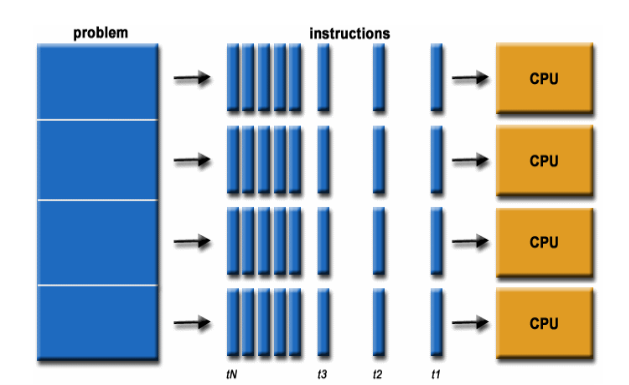
\includegraphics[width=\textwidth]{Images/Paralelo-ej1.png}
                  \caption{Ejemplo colas de supermercado, donde las \textbf{CPU} son las cajas donde cada familia, una por una procede a pagar por sus compras.}
                  \label{fig1:paralelo-ej1}
                \end{figure}
              \\\\En la figura \ref{fig1:paralelo-ej1} podemos ver \textbf {Problem} como la comida y productos de la familia, por otro lado, tenemos las \textbf{Instructions} como las personas en la cola, vemos el \textbf{CPU} como multiples cajeras atendiendo a las distintas familias al mismo tiempo.
              \\\\Vemos como una sola instrucción es ejectuda a la vez por un núcleo del \textbf{CPU}, aunque dispongamos en este caso de cuatro núcleos como nuestras cajeras.
              \\\\Cuando escribimos código, este en su proceso de compilación es ejecutado línea por línea.
              \\\\Al igual que la figura \ref{fig1:paralelo-ej1} vemos el programa siendo ejecutado, es decir, se compila y de esta forma se convierte en un proceso el cual, línea a línea es enviada a un núcleo del procesador para ser ejecutado.
              \\\\Podemos concluir que el \textbf{Procesamiento Paralelo} es un sistema con dos o mas procesadores conectados de tal manera que le sea posible compartir la ejecución de una determinda tarea.
%======================================================================
        \section{¿Qué es el Procesamiento Concurrente?}
          \subsection{Definición}
            \paragraph{Programación Concurrente}\mbox{} \\
              Siguiendo con la idea del supermercado, en este ejemplo tenemos una tienda con una única caja, pero varias filas.
              \\\\Partiendo de la figura \ref{fig2:paralelo-ej2} podemos ver \textbf {Problem} como la comida de la familia, y las \textbf{Instructions} como las personas en la cola.
                \begin{figure}[htb]
                \centering
                  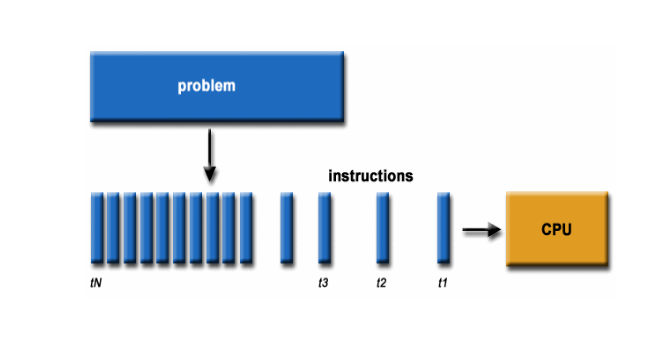
\includegraphics[width=\textwidth]{Images/Paralelo-ej2.png}
                  \caption{Ejemplo cola de supermercado, donde la \textbf{CPU} es la caja para pagar, y solo entra una familia a la vez a la caja.}
                  \label{fig2:paralelo-ej2}
              \end{figure}
              Y se ve el efecto de que un solo núcleo se ve asignado a un solo proceso.
              \\\\Se asigna un \textbf{Quantum}(esto signigica que se rotan por tiempo definido mediante un token, y este es asignado a cada uno de lo procesos, para nuestro ejemplo las personas serián los procesos).
            \\\\Por cada linea de código se presenta una instrucción que se ejecuta a la vez.
            \\Cuando compilamos código, los buses conectan todas las partes de un computador al procesador, y se hace el proceso de conversión de Alto nivel a Bajo nivel, hablamos de la conversión de código como programa a proceso mediante su interpretación en binario. Esto es un proceso línea a línea.
            \\\\Cuando hablamos de un computador tenemos:
             \begin{itemize}
               \item Partes
              \begin{enumerate}
                \item Periféricos de entrada y salida I/O
                \item Central Process Unit
                \item Random Access Memory
                \item Buses de Datos
              \end{enumerate}
             \end{itemize}\mbox{}\\
            \\El CPU recibe las señales de los buses, siendo así la manera como el procesador recibe entradas y salidas temporales o permanentes.
            \\Es importante aclarar sobre las arquitecturas de los procesadores, ya que existen de 32 bits y 64 bits.\\Tenemos que las arquitecturas de 32 bits cuentan con 32 buses de datos para comunicarse con el \textbf{CPU}, y las arquitecturas de 64 bits, cuentan con 64 buses de datos.
            \\Los procesadores como son máquinas hay que decirles cuando procesar, el \textbf{CPU} toma la información del disco que viaja mediante el bus en su velocidad de reloj para procesar, siendo esta la manera en que procesa la información del disco en el bus.
          \\Para procesar, el procesador tiene unos transistores y trabajan con sistemas Flip-Flop guardando los estados de 1 y 0.\\Estos son llamados Máquina de estado, donde se mueven los estados para conocer sus pulsos, y saber de esta manera entre los estados guardados la información que esta almacenada y escrita.
           \\\\Cuando hay muchos procesos cada uno es interpretado instrucción por instrucción hasta que finalice, la solución se logra dando uso a varios procesadores. Por esto, el \textbf{Procesamiento Paralelo} es más rapido.
           \\\\Luego tenemos el concepto \textit{Data Center}, donde hay muchos nodos de computo, siendo cada uno de estos computadores con procesadores disponibles.
           \\\\Un Data Center se comporta como una sola máquina, un solo servidor.
           \\Le podemos decir al Data Center que tenemos \textbf{10 Aplicaciones} durisimas, y esto supone un trabajo pesado en procesamiento, pero tenemos el Data center.
           \\Significa que podemos decirle a los procesadores que de manera \textbf{Paralela} se repartan la carga de la tarea. Por ejemplo, una carga de tarea pesada es el entrenamiento de un algoritmo de \textit{Inteligencia Artificial}.
           \begin{itemize}
             \item Conceptos importantes:
               \begin{enumerate}
                 \item \textbf{Quantum}: Tiempo limite que es S.O asigna a a ajecución de un proceso, transcurrido este se lasa al siguiente.
                 \item \textbf{Cambio de contexto}: Proceso llevado a cabo por el S.O para salvaguardar los datos actuales de ejecución del proceso.
               \end{enumerate}
           \end{itemize}
          Para el sistema operativo ejecutar procesos a la vez, les asigna un \textbf{Quantum}, y en ese tiempo asignado se ejecutan las intrucciones, cuando se acabe debe llegar al siguiente proceso y ejecutar sus instrucciones. Cuando termine se vuelve a asignar un nuevo \textbf{Quantum}.
          \\Para el sistema operativo salvaguardar los datos se utilizan punteros, cuando el Quantum finaliza se pone un puntero, "Se crea el Cambio de proceso" y se asigna un puntero para llevar el orden.
          \\\\La programación concurrente no produce mayor velocidad, podemos decir que es más lenta, puesto que hay que esperar un turno para ejecutar las intrucciones, pero en paralelo cada una de las intrucciones tienen su núcleo. Permite la programación concurrente lidiar con varias tareas al tiempo.
          \\El tiempo que se da al Quantum podría causar el efecto de lentitud y no se persive el efecto de concurrente, y si es muy pequeño no se logra ejecutar las intrucciones.
          \\De UNIX nacio la variante Linux, pero tenemos tambien Solaris y Windows, precisamente es dificil la creación de los sistemas operativos porque es dificil su depuración.
          \\Si no esta el puntero de donde comienza, vuelve a comenzar desde cero, y estos punteros son guardados en la RAM.
        \section{¿Qué es un Proceso?}
          \paragraph{}\mbox\\
            Para un proceso poder ejecutarse requiere de espacio de direcciones.
            \\Uno de los procesos del sistemas operativos es el cambio de contexto.
            Los procesos tiene varios estados, y no siempre estan en ejecución, ya que pueden estar en espera de un subproceso.


%----------------------------------------------------------------------

    \part{Computación en la nube}
    \part{Inteligencia Artificial}
    \part{IoT Intenet de las Cosas}
    \part{Big Data y Data Analytics}
%======================================================================
    \part{Metodología de Calificación}
      \chapter{Cortes}
        \section{Porcentajes evaluativos}
          \paragraph{Cortes 1, 2, 3}\mbox{}\\
          La metodología será para cada 15 días, ver las 2 horas por materia los días viernes.
            \begin{itemize}
              \item Corte 1
              \begin{enumerate}
                \item Talleres 10\%
                \item Proyecto 10\%
                \item Parcial 15\%
                \item Acumulado 35\%
              \end{enumerate}
              \item Corte 2
              \begin{enumerate}
                 \item Talleres 10\%
                \item Proyecto 10\%
                \item Parcial 15\%
                \item Acumulado 35\%
              \end{enumerate}
              \item Corte 3
              \begin{enumerate}
                \item Talleres 10\%
                \item Proyecto 10\%
                \item Parcial 15\%
                \item Acumulado 35\%
              \end{enumerate}
            \end{itemize}
%======================================================================
\end{document}

